\noindent
{\bf Collaborative Research: Mathematical modeling and simulation of
self-assembling amphiphilic particles in solvent} \\
{\em Rolf Ryham (lead PI, Fordham University),
Bryan Quaife (PI, Florida State University), and
Yuan-Nan Young (PI, New Jersey Institute of Technology)}

\section{Background}
\label{sec:background}
%The goal of this collaborative proposal is to use mathematical modeling
%and numerical simulations to investigate the dynamic self-assembly of
%amphiphilic particles interacting via hydrophobic forces in solvent.
This collaborative proposal aims to advance
the mathematical modeling and numerical simulation
of dynamic self-assembly of amphiphilic particles interacting
via hydrophobic forces in solvent.
Amphiphilic particles such as lipid molecules possess both hydrophobic
and hydrophilic structures. In a viscous solvent they self-assemble into
meso-/macroscopic structures such as micelles and bilayers of lipids to
shield their hydrophobic surfaces from contact with the solvent
molecules e.g., waters. Such self-assembly of amphiphiles via hydrophobic
forces is ubiquitous in biology~\cite{Israelachvili1954},
and has been a major source of nonspecific interactions 
in soft matter~\cite{Sanchez-IglesiasEtAl2012_ACSNano,
AltantzisEtAl2013_PSC, XieYangLuEtAl2020_COCIS}. 
%The proposed research aims to provide fundamental understanding of the
%self-assembly dynamics of amphiphilic particles so to design smart
%materials of desirable properties by
%tuning the geometry and properties of the amphiphilic particles. 

%The hydrophobic force arises when polar solvent molecules come in
%contact with a non-polar substance, such as hydrocarbon or vapor.
%In a polar solvent (like water), the dipole-dipole interaction between
%solvent molecules form a loosely structured hydrogen-bond network where
%each solvent molecule shares bonds with neighboring molecules at any
%given time \cite{Israelachvili1954}. In the presence of a non-polar
%solvent molecule loses the ability to form hydrogen bonds
%in one direction. 
%The decrease in the number of hydrogen bonds causes a reorientation,
%or structural change, in the surrounding water that is energetically
%very unfavorable \cite{Bjorneholm2016}.

\begin{wrapfigure}[15]{r}{0.37\textwidth}
\vspace{-8pt}
\centerline
{
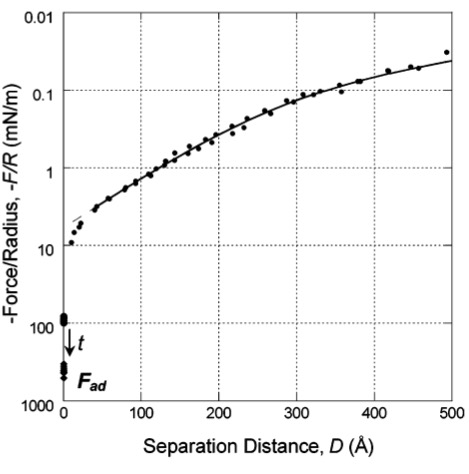
\includegraphics[width=0.36\textwidth]{figures/LongRangeForce.jpg}
}
%\vspace{-20pt}
\caption{\label{fig:force_distance}
Force-distance curve for surfactant
monolayers adsorbed on mica reveals a long-range
attraction~\cite{Lin2005}.}
\end{wrapfigure}

Macroscopically, the substantial free energy of placing hydrophobic
surfaces in contact with water is roughly proportional to the surface
area of the contact region~\cite{Bjorneholm2016}.
%As a result, hydrocarbon solutes have a large interfacial tension 
%and try to minimize their surface area when in water. 
At the microscopic level, however, there is long-range interaction
between hydrophobic surfaces. Two hydrophobic surfaces, in particular,
separated by water over some distance, experience an attraction
called the
hydrophobic force~\cite{Lum1999, Meyer2006, Hammer2010, KaScScNe16}.
The force is nonadditive~\cite{SilveraBatista1242477},
and measurements show that the hydrophobic force decays exponentially with a
decay length on the order of 1--10 nm~
\cite{Israelachvili1984,Marcelja1977,Christenson2001,Lin2005,Taetal13}
(Figure \ref{fig:force_distance}).


Motivated by its broad applicability to biology, chemistry, and engineering,
PIs RR and YNY developed a mathematical model, called the
hydrophobic attraction potential (HAP) model~\cite{Fu2018_SIAM},
that is based on
the linear response of water to surface perturbations. This model was
used by all the PIs to show how amphiphilic Janus particles (JP)
self-assemble into a vesicle-like structure~\cite{FuQuRyYo20}.
Janus particles are typically spherical particles with a biphasic
material label on either hemisphere \cite{CaFaRaVe89,Gaetal13,Mallory2017,HaBr20,McBr21}.
Based on
preliminary results (\S\ref{sec:preliminary_work}), the PIs propose to
extend this HAP model as a general methodology that leads
to new mathematical ideas and efficient numerical methods.

\subsection{Hydrophobic attraction}
The hydrophobic attraction potential theory concerns the self-organization of
hydrophobic particles in a viscous solvent. It is a phenomenological
model mimicking the linear-response of water to surface perturbations
and stems from work of Stjepan Mar\v{c}elja
from the Australian National University in 1976. To explain certain
repulsion measurements between lecithin bilayers, Mar\v{c}elja and
coworkers devised a mathematical model using a Landau expansion of the
free energy density of an order parameter for the orientation of
water~\cite{LeRaPa77, MaRa76, LANDAULIFSHITZ5}. Their truncated free
energy gave a boundary value problem for water structure that was
readily solved in terms of hyperbolic trigonometric functions. 

Although schematic, the model was general enough to explain a number of
physical effects. For example, the repulsion of lecithin bilayers
was explained by the free energy that decreases with distance of
separation because of the mean orientations of water being opposite at
the two interfaces. Later, a long-range attractive force between
hydrocarbon coated mica sheets was measured up to
100~nm~\cite{ClCh88,RaDe88}. The Mar\v{c}elja
theory was then applied to this problem for an order parameter
representing the excess number of hydrogen bonds per water
molecule and gave agreement with the measured force
curves~\cite{ErLjCl89}.


Analogues of Mar\v{c}elja's phenomenological theory appeared in other
areas related to biological self-assembly, such as interactions of
membrane-bound proteins~\cite{KoNa15, Nagle17, KUZMIN2005} and the
theory of polymer bead interaction in mixed solvents~\cite{deGe76}. On
the downside, it applies a continuum theory to distances of a few
molecular diameters, the association of order parameter is arbitrary, it
predicts monotonic forces, and finally the theory does not account for
the amplification in attraction at very short distances~\cite{Ni80}.

\begin{wrapfigure}[21]{l}{0.3\textwidth}
  \vspace{-5pt}
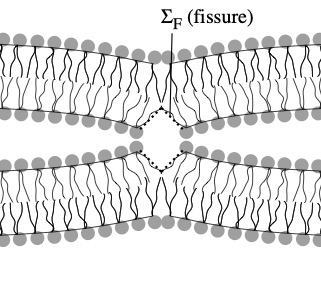
\includegraphics[width=0.3\textwidth]{figures/Fissure.jpg}
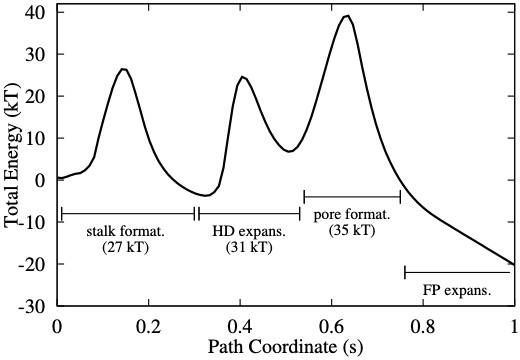
\includegraphics[width=0.3\textwidth]{figures/Landscape.jpg}
\caption{\label{fig:fissure} In fusion, fissures in the phospholipid
  monolayers expose hydrocarbon to water (top). The energy of fissures
  dominates first and third stages of fusion (bottom).
}
\end{wrapfigure}
Despite the ubiquity of
the phenomenon, theoretical developments explaining the basic underlying
principles of the hydrophobic effect have come relatively
late~\cite{Ch05}.
No single theory has been able to account, either qualitatively
or quantitatively,
for hydrophobic interaction over the full distance
regime~\cite{Lum1999, Lin2005, Meyer2006, Ducker2016}.
For example, studies of the partitioning of
hydrophobic solutes provide estimates for the energy cost of creating
hydrophobic-water contacts
that is a factor of three lower than the value derived from interfacial
tension measurements. Only recently was an explanation for this
discrepancy provided~\cite{Jackson2016}.

The continuum approach to water structure
that we present here is justified
\textit{a posteriori} by the agreement between theory and experiment.
Researchers have used Mar\v{c}elja's theory to calculate
energies of pore formation and fusion~\cite{Gletal88, Aketal17,
RyKlYaCo16}.
%When open, the attraction between apposing hydrophobic
%surfaces causes the fissure to collapse.
PI RR calculated a least energy path 
of fusion using a modified form of the Helfrich energy that
included Mar\v{c}elja's free energy for the structure of water
separating fissures~\cite{RyKlYaCo16} (Figure~\ref{fig:fissure}).
The calculated barrier heights were 
corroborated experimentally \cite{FrRoPi17}. In summary,
there is a consensus that despite its apparent simplicity, the predictions
of the hydrophobic attraction potential theory are compatible with
experimental measurements and may closely mirror the reality of
the physical process at a molecular scale~\cite{FrRoPi17, Fretal21}.

The HAP is a conceptual advance for modeling bilayer membranes.
Continuum elastic energies of membrane assume an energy density that
depends quadratically on the bilayer strain
\cite{Hamm2000,TerziDeserno17, PhysRevE.102.042406}.  The coefficients
of the continuum ansatz correspond to experimentally measured elastic
moduli \cite{Nagle17, Nagle17-2, NAGLE2000159}.  The HAP approach can
potentially explain membrane properties from first principles because it
derives elastic energies assuming parameters for the water structure and
particle shape \cite{Fu2018_SIAM, FuQuRyYo20, doi:10.1063/5.0009734,
LiAn-Chang16}.  Immersed boundary and boundary integral are highly
effective for modeling intact, giant unilamellar vesicles (GUV) because
they use relatively large time-step sizes and mesh sizes
\cite{
Shravan09,
Rahimian15,
KimLai2010_JCP,
KimLai2012_PRE,
HuLaiSeolEtAl2016_JCP,
Bartels,
Peng13,
RyKlYaCo16,
Sinha15,
Lowengrub13,
Hu,
Hu13}.
Conversely, the number of coarse-grained particles needed to track a GUV
in the HAP formalism is relatively large.  For microscopic process like
fusion, however, membrane deformations occur at a length scale
comparable to the thickness of the membrane
\cite{Kuzmin7235,Aeffner2012,KoKo2002}.  The small deformation
assumption of continuum theory no longer holds
\cite{Hamm2000,TerziDeserno17, PhysRevE.102.042406}.  The HAP theory
does encode membrane thickness through particle diameter, and it is
comparatively straightforward to account for proteins and lipid mixtures
by including several particle species.  Any ruptures or insertions occur
self-consistently in the HAP formulation.  Phase-field and level-set
methods also allow for topological changes but they require multiple
phase fields and level sets and additional (sometimes empirical) laws to
couple them to model membrane-membrane interactions
\cite{
DuLiuWang2004_JCP,
BibenKassnerMisbah2005_PRE,
DoyeuxGuyotChabannesEtAl2013_JCAM,
Du05,
QiangDu08,
doi:10.1098/rspa.2012.0505,
doi:10.1137/130941432,
Feetzl18,
doi:10.1137/16M1108406}.
In addition, these methods require the entire fluid and interfacial
domains to be discretized.  In contrast, the HAP methodology allows
evolution equations to be solved using integral equation methods that
when optimized have linear or near-linear computational complexity in
the number of particles~\cite{fmm1, fmm2, fmm3, fmm4, fmm5, fmm6, fmm7,
fmm8}.


